\documentclass[a4paper, 12pt]{article}
% packages
\usepackage{amssymb}
\usepackage[fleqn]{mathtools}
\usepackage{tikz}
\usepackage{enumerate}
\usepackage{bussproofs}
\usepackage{xcolor}
\usepackage[margin=1.3cm]{geometry}
\usepackage{logicproof}
\usepackage{diagbox}

% augmented matrix
\makeatletter
\renewcommand*\env@matrix[1][*\c@MaxMatrixCols c]{%
\hskip -\arraycolsep
\let\@ifnextchar\new@ifnextchar
\array{#1}}
\makeatother

% ceiling / floor
\DeclarePairedDelimiter{\ceil}{\lceil}{\rceil}
\DeclarePairedDelimiter{\floor}{\lfloor}{\rfloor}

% custom commands
\newcommand{\indefint}[2]{\int #1 \, \mathrm{d}#2}
\newcommand{\defint}[4]{\int_#1^#2 #3 \, \mathrm{d}#4}
\newcommand{\dif}[2]{\frac{\mathrm{d}#1}{\mathrm{d}#2}}
\newcommand{\limit}[2]{\displaystyle{\lim_{#1 \to #2}}}
\newcommand{\summation}[3]{\sum\limits_{#1}^#2 #3}
\newcommand{\intbracket}[3]{\left[#3\right]_#1^#2}

\newcommand{\powerset}[0]{\wp}
\renewcommand{\emptyset}[0]{\varnothing}

\newcommand{\unaryproof}[2]{\AxiomC{#1} \UnaryInfC{#2} \DisplayProof}
\newcommand{\binaryproof}[3]{\AxiomC{#1} \AxiomC{#2} \BinaryInfC{#3} \DisplayProof}

% no indent
\setlength\parindent{0pt}

% reasoning proofs
\newcommand{\proofline}[3]{(#1)\ & #2 & \text{#3} \\}
\allowdisplaybreaks

% actual document
\begin{document}
    \section*{CO150 - Graphs and Algorithms}
        \subsection*{Prelude}
            The content discussed here is part of CO150 - Graphs and Algorithms (Computing MEng); taught by Iain Phillips, in Imperial College London during the academic year 2018/19. The notes are written for my personal use, and have no guarantee of being correct (although I hope it is, for my own sake). This should be used in conjunction with the notes.
        \subsection*{14th January 2019}
            Introduction to the structure of the course;
            \begin{enumerate}[{Part} I:]
                \itemsep0em
                \item Graphs
                \item Graph Algorithms
                \item Algorithm Analysis
                \item Introduction to Complexity
            \end{enumerate}
            An example graph with a real life application;
            \begin{center}
                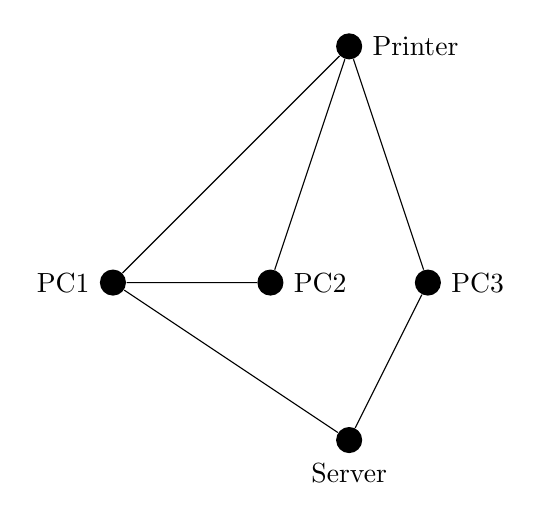
\begin{tikzpicture}
                    \node[circle, fill=black, label=right:PC2] (pc2) at (0, 0) {};
                    \node[circle, fill=black, label=left:PC1] (pc1) at (-2, 0) {};
                    \node[circle, fill=black, label=below:Server] (server) at (1, -2) {};
                    \node[circle, fill=black, label=right:PC3] (pc3) at (2, 0) {};
                    \node[circle, fill=black, label=right:Printer] (print) at (1, 3) {};

                    \draw
                    (print) -- (pc1)
                    (print) -- (pc2)
                    (print) -- (pc3)
                    (server) -- (pc1)
                    (server) -- (pc3)
                    (pc1) -- (pc2);
                \end{tikzpicture}
            \end{center}
            Note how all the PCs are directly connected to the printer, but PC2 can only reach the server through PC1.
\end{document}
